\documentclass[tikz,border=5pt]{standalone}
\usepackage{tikz}
\usetikzlibrary{arrows.meta,decorations.pathmorphing,patterns}

% Atlas color palette
\definecolor{AtlasTeal}{HTML}{5BA4A4}
\definecolor{AtlasWarm}{HTML}{C17F59}
\definecolor{AtlasSage}{HTML}{7A9E7E}
\definecolor{AtlasWarmLight}{HTML}{F0DED3}

\begin{document}
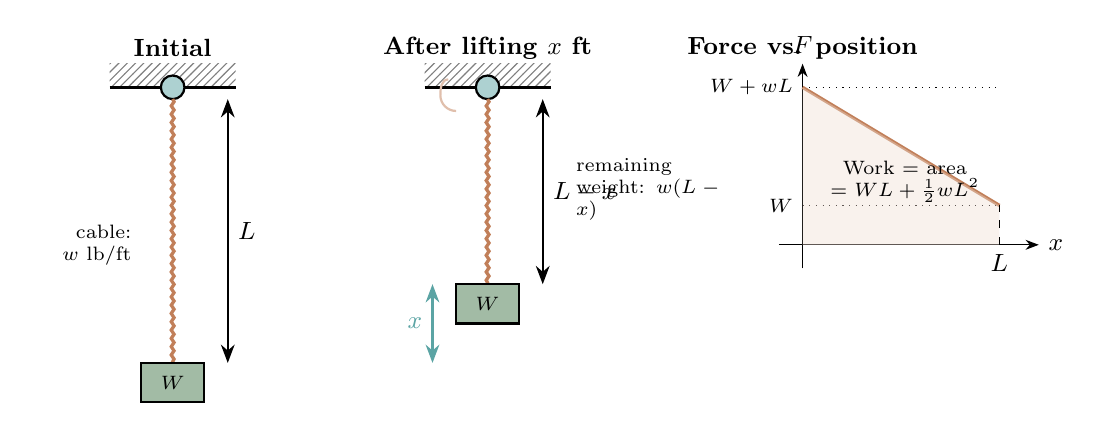
\begin{tikzpicture}[>=Stealth]
    
    % ========== LEFT: Initial state ==========
    \begin{scope}[shift={(-2.5,0)}]
        \node[font=\bfseries\small] at (0,4.5) {Initial};
        
        % Top platform
        \fill[pattern=north east lines, pattern color=gray] (-0.8,4) rectangle (0.8,4.3);
        \draw[very thick] (-0.8,4) -- (0.8,4);
        
        % Pulley suggestion
        \fill[AtlasTeal!50] (0,4) circle (0.15);
        \draw[thick] (0,4) circle (0.15);
        
        % Cable/rope (full length)
        \draw[AtlasWarm, very thick, decorate, decoration={snake, amplitude=0.5pt, segment length=3pt}] 
            (0,3.85) -- (0,0.5);
        
        % Weight at bottom
        \fill[AtlasSage!70] (-0.4,0) rectangle (0.4,0.5);
        \draw[thick] (-0.4,0) rectangle (0.4,0.5);
        \node[font=\scriptsize] at (0,0.25) {$W$};
        
        % Length annotation
        \draw[<->, thick] (0.7,0.5) -- node[right, font=\small] {$L$} (0.7,3.85);
        
        % Cable weight annotation
        \node[left, font=\scriptsize, text width=1.2cm, align=right] at (-0.4,2) 
            {cable: $w$ lb/ft};
    \end{scope}
    
    % ========== MIDDLE: Partially lifted ==========
    \begin{scope}[shift={(1.5,0)}]
        \node[font=\bfseries\small] at (0,4.5) {After lifting $x$ ft};
        
        % Top platform
        \fill[pattern=north east lines, pattern color=gray] (-0.8,4) rectangle (0.8,4.3);
        \draw[very thick] (-0.8,4) -- (0.8,4);
        
        % Pulley
        \fill[AtlasTeal!50] (0,4) circle (0.15);
        \draw[thick] (0,4) circle (0.15);
        
        % Lifted cable (coiled on top - suggestion)
        \draw[AtlasWarm!50, thick] (-0.5,4.1) to[out=180,in=90] (-0.6,3.9) 
            to[out=-90,in=180] (-0.4,3.7);
        
        % Remaining hanging cable
        \draw[AtlasWarm, very thick, decorate, decoration={snake, amplitude=0.5pt, segment length=3pt}] 
            (0,3.85) -- (0,1.5);
        
        % Weight (higher)
        \fill[AtlasSage!70] (-0.4,1) rectangle (0.4,1.5);
        \draw[thick] (-0.4,1) rectangle (0.4,1.5);
        \node[font=\scriptsize] at (0,1.25) {$W$};
        
        % x distance lifted
        \draw[<->, thick, AtlasTeal] (-0.7,0.5) -- node[left, font=\small] {$x$} (-0.7,1.5);
        
        % Remaining length
        \draw[<->, thick] (0.7,1.5) -- node[right, font=\small] {$L-x$} (0.7,3.85);
        
        % Current weight annotation
        \node[right, font=\scriptsize, text width=2cm] at (1,2.7) 
            {remaining weight: $w(L-x)$};
    \end{scope}
    
    % ========== RIGHT: Force diagram ==========
    \begin{scope}[shift={(5.5,2)}]
        \node[font=\bfseries\small] at (0,2.5) {Force vs. position};
        
        % Axes
        \draw[->] (-0.3,0) -- (3,0) node[right, font=\small] {$x$};
        \draw[->] (0,-0.3) -- (0,2.3) node[above, font=\small] {$F$};
        
        % Initial force (W + wL)
        \node[left, font=\scriptsize] at (0,2) {$W + wL$};
        \draw[dotted] (0,2) -- (2.5,2);
        
        % Final force (just W)
        \node[left, font=\scriptsize] at (0,0.5) {$W$};
        \draw[dotted] (0,0.5) -- (2.5,0.5);
        
        % Force decreases linearly (cable part)
        \draw[AtlasWarm, very thick] (0,2) -- (2.5,0.5);
        
        % Work = area under curve
        \fill[AtlasWarmLight, opacity=0.4] (0,0) -- (0,2) -- (2.5,0.5) -- (2.5,0) -- cycle;
        
        % L marker
        \node[below, font=\small] at (2.5,0) {$L$};
        \draw[dashed] (2.5,0) -- (2.5,0.5);
        
        % Work annotation
        \node[font=\scriptsize, text width=2cm, align=center] at (1.3,0.8) 
            {Work = area\\$= WL + \frac{1}{2}wL^2$};
    \end{scope}

\end{tikzpicture}
\end{document}
